% !TEX encoding = UTF-8 Unicode
% !TEX spellcheck = en-US
\documentclass[
    aps,
    prl,
    showkeys,
    nofootinbib,
    %twocolumn,
    floatfix
]{revtex4-1}

\usepackage[utf8]{inputenc} % UTF-8
\usepackage{braket}

\usepackage{amsmath}
\usepackage{amssymb}

\usepackage{graphicx}

\renewcommand{\vec}[1]{\boldsymbol{#1}}


\newcommand{\fm}{\,\mathrm{fm}}
\newcommand{\ifm}{\,\mathrm{fm}^{-1}}
\newcommand{\MeV}{\,\mathrm{MeV}}

\begin{document}

\title{Discretization}

\author{C.~Körber}

\date{\today}

\begin{abstract}%
	How does the contact interaction depend on discretization effects?
\end{abstract}

\maketitle

\section{No discretization}
\subsection{1-d}
\subsubsection{Positive energies}

The momentum space Schrödinger equation
\begin{equation}
	\frac{p^2}{2 \mu} \psi(p) + \int \frac{d p}{2\pi} \braket{p | \hat V | p'} \psi(p') = E \psi(p')
\end{equation}
for contact interactions this becomes
\begin{equation}
	\frac{p^2}{2 \mu} \psi(p) +  c I_0 = E \psi(p') \, , \qquad I_0 = \int \frac{d p'}{2\pi} \psi(p') \, .
\end{equation}
Thus
\begin{equation}
	\psi(p) = \frac{c I_0}{E - \frac{p^2}{2\mu}}
\end{equation}
For scattering solutions we need $i\epsilon$ prescription
\begin{align}
	I_0 &= \int \frac{d p}{2\pi}  \frac{c I_0}{E - \frac{p^2}{2\mu} + i \epsilon} \\
	&= I_0 \times \frac{\mu c }{\pi} \int\limits_{ - \infty}^{\infty} \frac{d p}{\gamma^2 - {p^2} + i \tilde\epsilon} \, , \quad \gamma^2 = 2 \mu E > 0\,.
\end{align}
The remaining integral can be solved by the residual theorem: the zeros of the denominator are
\begin{align}
	\gamma^2 - {p^2} + i \tilde\epsilon &= (\gamma + i \tilde\epsilon - p)(\gamma + i \tilde\epsilon + p) \, .
\end{align}
Note that the zeros are independent on the sign of $\epsilon$ (one root in upper and one root in lower plane).
Completing the integral in the upper plane selects the residual $p_0 = \gamma + i \tilde \epsilon$ and thus
\begin{equation}
	\int\limits_{ - \infty}^{\infty} \frac{d p}{\gamma^2 - {p^2} + i \tilde\epsilon}
	=
	 \frac{2 \pi i}{2 \gamma} \, .
\end{equation}
and therefore
\begin{equation}
	1 = \frac{\mu c}{\pi} \times \frac{\pi i}{\gamma} \, ,
\end{equation}
or
\begin{equation}
	\gamma = i \mu c \, \Rightarrow  E = - \frac{\mu c^2}{2}
\end{equation}
In other words, you do not get positive energies for $c \in \mathbb{R}$.

It seems like, you only get positive energies once you are in a box...

\clearpage
\section{Understanding the unitary limit}


From my understanding, the unitary limit appears when the total cross section is independent of microscopic parameters.
The cross section is given by
\begin{equation}
	\frac{d \sigma}{d \Omega} = | f(\Omega, p) | ^ 2 \, ,
\end{equation}
where
\begin{align}
	f(\Omega, p) &= \sum_{l=0}^{\infty} f_l(\Omega, p) \, , \\ 
	f_l(\Omega, p) &\sim g_l(\Omega) \times \left[\exp( 2 i \delta_l (p)) - 1\right]
\end{align}
This is generally true for all $d = 1, 2, 3$ cases modulo not important factors.

In our system, for a simple contact interaction of strength $c_0$, we only find contributions to $l=0$.
Regarding your eq. (7), one finds that
\begin{equation}
	\cot \delta_0 (p) = \begin{cases}
		a_0 p &, \, d = 1 \\
		2 / \pi \log(a_0 p) &, \, d = 2 \\
		- 1/(a_0 p) &, \, d = 3
	\end{cases}
\end{equation}

In other words, we are at the unitary limit if $\cot \delta_0$ is independent of $a_0$.
This can only happen if $a_0 \rightarrow \infty$ or $a_0 \rightarrow \pm 0$ because $a_0$ must be independent of $p$.

\textbf{Does this make sense?}

To discriminate between infinite volume and lattice, I will label the momentum points which are extracted from lattice (as in continuum but finite volume) as $\gamma_i$.
Here, $\gamma_i^2 = 2 \mu E_i$, $\mu$ being the reduced two-particle mass and $E_i$ being the lattice energy spectrum.

Using your equations (35-37) and combining this with your eq. (7), one finds
\begin{equation}\label{def:a0}
	a_0 = \begin{cases}
		\frac{L}{2\pi^2}S_1(x_i) & \, , d =1 \\
		\frac{L}{2\pi} \exp \left\{ S_2(x_i) / (2\pi) \right\} & \, , d =2 \\
		\frac{ \pi L}{ S_3(x_i) } & \, , d =3
	\end{cases}
	\qquad \forall_i \, ,
\end{equation}
with $S_j(x_i)$ being the Lüscher Zeta function in $j$ dimensions and $ x_i = \mu E_i L ^2 / (2 \pi^2) $.
In other words, if your computation does the right thing, you fix your contact interaction strength $c_0$, which will give you a set of energy levels $E_i(c_0)$.
For all of the eigenstates $E_i$, all points $S_j(x_i)$ lay on a line because, because $a_0$ is independent of the energy level and eq.~\eqref{def:a0} tells us that there is a one-to-one relation between $S_j(x_i)$ and $a_0$.

So in which cases do we find that $a_0 \to 0, \pm \infty$?

\begin{itemize}
	\item For $d = 1$ find $c_0$ such that $S_1(x_i(c_0)) \to 0, \pm \infty$ $\forall_i$.
		Regarding your plots,
		\begin{itemize}
			\item $S_1(x_i(c_0)) = 0$ is not possible $\forall_i$ (ground state only approaches zero).
			\item $S_1(x_i(c_0)) \to - \infty$ is not possible $\forall_i$ (ground state $>0$).
			\item $S_1(x_i(c_0)) \to + \infty$ is possible $\forall_i$ if $c_0 \to 0^-$.
		\end{itemize}
	\item For $d = 2$ find $c_0$ such that $S_2(x_i(c_0)) \to + \infty$ $\forall_i$.
		Regarding your plots,
		\begin{itemize}
			\item $S_2(x_i(c_0)) \to + \infty$ is possible for $c_0 \to 0^-$.
		\end{itemize}
	\item For $d = 3$ find $c_0$ such that $S_3(x_i(c_0)) \to 0, \pm \infty$ $\forall_i$.
		Regarding your plots,
		\begin{itemize}
			\item $S_3(x_i(c_0)) = 0$ is possible $\forall_i$.
			\item $S_3(x_i(c_0)) \to \pm \infty$ is possible for $c_0 \to 0^\mp$.
		\end{itemize}
\end{itemize}

Obviously, the cases for $c_0 \to 0^\pm$ make sense --- if there is no interaction, than there is only the mass scale.
However this solution is not of interest.
This leaves $d=3$ as the only interesting case.

\newpage
\section{Momentum Space confusion}
This is a non complete description!
It should serve as a summary.

As we figured out most recently, it is interesting to look at Lüschers equation in a discrete finite volume if you want to connect discrete finite energy levels with continuum infinite volume phase shifts.
If you don't do so, you find that the discretization (in a finite volume) apparently induces an effective range (see figure \ref{fig-cont-lusch}).
\begin{figure*}[!htb]
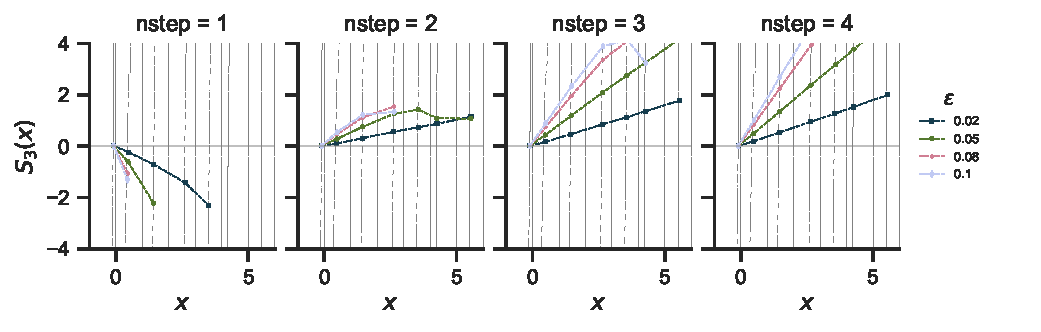
\includegraphics[width=0.9\textwidth]{figs/eff-range-cont-lusch.pdf}
\caption{
    \label{fig-cont-lusch}Phase shifts extracted from continuum Lüscher equation for discrete finite volume eigenvalues of contact interaction Hamiltonian.
    The contact interactions was chosen such that the ground state matches the first zero of the zeta function.
    $\epsilon$ is the lattice spacing in [fm] for a box of size $L = 1$ [fm].
    $n_{\mathrm{step}}$ describes the implementation of the Laplace derivative.
    E.g., $n_{\mathrm{step}} = 1$ corresponds to an one step derivative where corrections are expected to scale with $\epsilon^2$.
    The variable $x$ is directly proportional to the eigenvalues of the Hamiltonian $x = 2 \mu E L^2 / (2 \pi)^2$.
    Even thought the interaction has no effective range (contact interaction), the effective range expansion for more precise implementations of the derivative, certainly is proportional to $x$.
 }
\end{figure*}

The trick you have used to get there was to replace the finite volume continuum Zeta function .
\begin{equation}
    S_3(x) = \sum\limits_{\vec n \in M(\Lambda)} \frac{1}{\vec n ^2 - x} - 4 \pi \Lambda
    \, , \qquad
    M(\Lambda) = \left\{ \vec n \in \mathbb N \middle\vert 0 \leq n_i \leq \Lambda \right\}
\end{equation}
with a "discretized version"
\begin{equation}
    \mapsto
    S_3^{\mathrm{lat}}(x) = \frac{4 \pi^2}{L^2} \sum\limits_{\vec k \in M^\epsilon(L)} \frac{1}{\vec k ^2 - 2 \mu E} - \mathcal L \pi^2 \frac{L}{\epsilon}
    \, , \qquad
    M^\epsilon(L) = \left\{ \vec k \in \frac{2 \pi}{L} \mathbb N \middle\vert - \frac{\pi}{\epsilon} \leq k_i < \frac{\pi}{\epsilon} \right\}
    \, ,
\end{equation}
where $\mathcal L = 0.777551 \cdots$ is the normalization of the momentum integral and the sum is limited but the momentum cutoff of the discrete spatial lattice.

This certainly improved the effective range expansion (see fig.~\ref{fig-cont-lusch}).
\begin{figure*}[!htb]
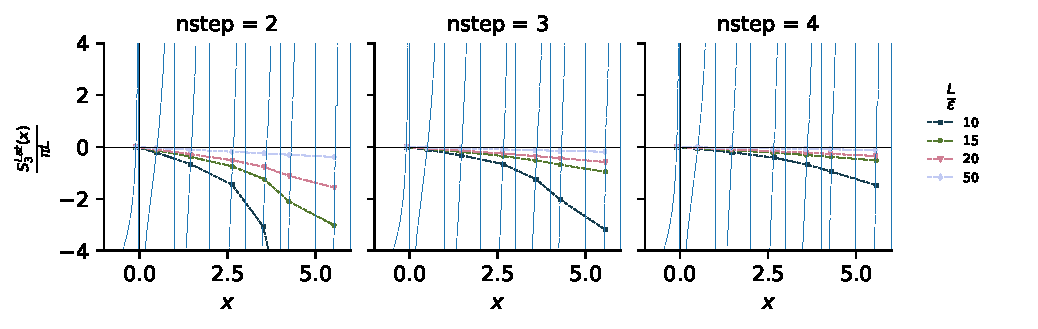
\includegraphics[width=0.9\textwidth]{figs/eff-range-discrete-lusch.pdf}
\caption{
    \label{fig-cont-lusch}Phase shifts extracted from discrete Lüscher equation for discrete finite volume eigenvalues of contact interaction Hamiltonian.
    $\epsilon$ is the lattice spacing in [fm] for a box of size $L = 1$ [fm].
 }
\end{figure*}

Even thought the utilization of the discrete Lüscher equation improves the description, e.g., reduces the size of the induced effective range, the results are not perfectly constant (e.g., equal to zero because of the choice of the contact interaction).
On top of that, we now see curvature in the effective range expansion.
This might be still the cause of further discretization effects.
Next, I describe how one can improve on that.

\subsection{Removing all discretization effects -- making ERE flat}
\textbf{The idea:} Implement an exact discrete derivative by transforming to momentum space, multiplying by the exact $p^2$, and transforming back to coordinate space.
Doing so, remove all derivative discretization approximations and hopefully recover a flat effective range expansion.

\textbf{The conclusion:} This is not possible.

\textbf{The next step:} Implementing the "actual" discrete Lüscher equation.

\subsubsection{The idea}
The idea is straight forward:

\begin{equation}
	\braket{ \vec r ' | \hat H_0 | \vec r}
	=
	\int d \vec q^3 \int d \vec k^3 \braket{ \vec k | \hat H_0 | \vec q} \braket{\vec r' | \vec k} \braket{\vec q | \vec r}
	=
	\int d \vec q^3 H_0(\vec q) \exp\left\{ i \vec q \cdot \left( \vec r - \vec r '\right)\right\}
\end{equation}
Discrete FFTs are already implemented in python, so the only remaining challenge is to multiply the transformed input times the expectation values of the kinetic Hamiltionian $H_0(\vec q)$.

But this turned out to be a major source of confusion.
As an example, suppose you have four spatial sites in a one dimensional discrete box with periodic boundary conditions.
This means, your momenta are discrete $\ket{\vec p} = \ket{2 \pi / L \vec n}$ with $\vec n \in \mathbb Z^3$ and periodic  $\ket{\vec p + 2 \pi / \epsilon} = \ket{\vec p}$.
A possible choice for momentum basis states are
\begin{equation}
	B_1(L = 4\epsilon, \epsilon)
	= \left\{ \frac{2\pi}{4\epsilon} \times n \middle \vert n \in \{-2, -1, 0, 1\} \right\}
	= \left\{ -\frac{\pi}{\epsilon}, -\frac{\pi}{2\epsilon}, 0, \frac{\pi}{2\epsilon} \right\} \, .
\end{equation}
The naive choice of eigenvalues are thus
\begin{equation}
    H(B_1) = \frac{1}{2\mu} \frac{\pi^2}{4 \epsilon^2} \left\{ 4, 1, 0, 1\right\} \, .
\end{equation}
But because of the periodicity of momenta $\ket{\vec p} = \ket{\vec p + 2\pi/\epsilon}$, the following basis is a valid choice as well:
\begin{equation}
	B_2(L = 4\epsilon, \epsilon)
	= \left\{ \frac{2\pi}{4\epsilon} \times n \middle \vert n \in \{0, 1, 2, 3\} \right\}
	= \left\{ 0, \frac{\pi}{2\epsilon}, \frac{\pi}{\epsilon}, \frac{3\pi}{2\epsilon} \right\} \, , \qquad
	H(B_2) = \frac{1}{2\mu} \frac{\pi^2}{4 \epsilon^2} \left\{ 0, 1, 4, 9\right\} \, .
\end{equation}
And since the discrete Fourier transformations are unitary transformations (and thus the eigenvalues of the Hamiltonian do not change through FTs), clearly the different implementations of the Hamiltonian return different answers.

Most interestingly, when actually implementing a 1-step derivative and running the FFTs in python, the first basis is actually preferred.

What's happening?

You have to manually take care of the periodicity!
Look at coordinate space.
Lüscher actually defines his finite volume periodic boundaries operators such that
\begin{equation}
    O_L(\vec r) = O_L(\vec r + \vec n L) = \frac{1}{\mathcal N} \sum _{\vec n \in \mathbb Z} O(\vec r + \vec n L)\, ,
\end{equation}
where $\mathcal N$ is a normalization and the infinite volume operator has a finite range such that $\lim\limits_{L\to \infty} O_L(\vec r) = O(\vec r)$.

So, how do we do the same thing for momenta.
The answer is basically the same.
Implement the expectation values of the operators such that
\begin{itemize}
    \item[(A)] The operators $O_\epsilon$ are periodic in $\frac{2\pi}{\epsilon}$ and
    \item[(B)] In the limit of $\epsilon \to 0$, you obtain  $O_\epsilon \to  O$.
\end{itemize}

So what's a valid choice?
\begin{equation}
	D^1( \vec p, \epsilon) = \sum_{i=1}^3 \frac{2 - 2 \cos(\epsilon p_i)}{\epsilon^2} \, .
\end{equation}
That's just the same thing you would do in coordinate space by introducing a finite step derivative.
In principal you can also do better and implement improved operators for faster convergence.

In other words: a naive infinite order improvement is not possible -- it does not matter where or how you implement your derivative.
If you take care of discretization and periodic boundary conditions, there is always a one to one correspondence of momentum and coordinate space.
At some point, it might be more efficient numerically though to run computations in one or the other space...

But here is the actual catch: since the momentum dispersion relation you have used $D^\infty(\vec p, \epsilon) = \vec p^2$ is actually not obtainable on a lattice (unless $n_{\mathrm{step}} \to \infty$), you should use the actual lattice dispersion relation (spectrum of $H_0$) to execute the Lüscher sum.

\subsection{New equations}

What I am suggesting is that the new equations are the following:
Instead of the infinitely improved dispersion relation $D^\infty(\vec p, \epsilon)$ (which is the continuum dispersion relation in a fixed interval), you should use the discrete lattice dispersion relation
\begin{equation}
    D^\infty(\vec p, \epsilon) = \vec p ^2 
    \to 
    D^{n_{\mathrm{s}}}(\vec p, \epsilon) 
    =
    \frac{1}{\epsilon^2} \sum\limits_{i=1}^3 \sum\limits_{n_i=-n_{\mathrm{s}}}^{n_{\mathrm{s}}} c_{|n_i|}^{n_{\mathrm{s}}} \cos( p_i n_i \epsilon)
\end{equation}
Where the coefficients $c_i^{n_{\mathrm{s}}}$ are enforced by the constrained
\begin{equation}\label{def:lattice-dispersion}
    D^{n_{\mathrm{s}}}(\vec p, \epsilon)
    =
    p^2 + \mathcal O \left(\epsilon^{2 n_{\mathrm{s}}}\right)
    \, .
\end{equation}
A few coefficients are given in table \ref{tab-dispersion-coeff}.

\begin{table}[htb]
\centering
\begin{tabular}{r | ccccc}
$ c_{i}^{n_{\mathrm{s}}}$ & i = 0 & 1 & 2 & 3 & 4 \\ \hline
$n_{\mathrm{s}} = 1$ & 2 & -1 \\
2 & $\frac{5}{2}$ & $-\frac{4}{3}$ & $\frac{1}{12}$ \\
3 & $\frac{49}{18}$ & $-\frac{3}{2}$ & $\frac{3}{20}$ & $-\frac{1}{90}$ \\
4 & $\frac{205}{72}$ & $-\frac{8}{5}$ & $\frac{1}{5}$  & $-\frac{8}{315}$ & $\frac{1}{560}$
\end{tabular}
\caption{\label{tab-dispersion-coeff}Coefficients for discrete momentum dispersion relation.
    Note that this coefficients are minus the Laplace finite step coefficients (because $\partial_x^2 \leftrightarrow - p^2$).
}
\end{table}

Thus one has to update the counter term in the zeta function definition (your $m = 2\mu$) (do I get the factors right)
\begin{equation}
    \frac{\pi}{\epsilon}
    \mathcal L
    =
    \frac{4 \pi}{(2\pi)^3}
    \left(
    \prod \limits_{i=1}^3
    \int\limits_{-\pi /\epsilon}^{\pi / \epsilon}
    d q_i
    \right)
    \frac{1}{q_1^2 + q_2^2 + q_3^2}
    \to
    \frac{4 \pi}{(2\pi)^3}
    \left(
    \prod \limits_{i=1}^3
    \int\limits_{-\pi / \epsilon}^{\pi / \epsilon}
    d q_i
    \right)
    \frac{1}{D^{n_{\mathrm{s}}}(\vec p, \epsilon)}
\end{equation}
and adjust the zeta function
\begin{equation}
    S_3^{\mathrm{lat}}(x) = \frac{4 \pi^2}{L^2} \sum\limits_{\vec k \in M^\epsilon(L)} \frac{1}{\vec D^{n_{\mathrm{s}}}(\vec p, \epsilon) - 2 \mu E} - \mathcal L \pi^2 \frac{L}{\epsilon}
    \, , \qquad
    M^\epsilon(L) = \left\{ \vec k \in \frac{2 \pi}{L} \mathbb N \middle\vert - \frac{\pi}{\epsilon} \leq k_i < \frac{\pi}{\epsilon} \right\}
    \, ,
\end{equation}

Let me know what you think about that.

\newpage
\section{Long Range Forces}
Long range potentials defined by non-zero effective range and higher ERE parameters are the next step in the direction of realistic nuclear potentials.
Is it possible to improve the lattice finite volume effective range expansion for long range forces in the same manner as in the unitary case?
Particularly, if length scales like a non-zero scattering length and effective range are present, how do they mix with induced length scales?
Is there a power counting in terms of induced over physical quantities?

It is desirable to choose a potential where the infinite volume continuum results can be computed analytically, to answer the above questions in the most accurate way.
For this reason, I have choosen the following separable potential
\begin{align}
	V(\vec p', \vec p) &= - g^*(\vec p') g(\vec p) \, ,
	&
	g(\vec{p})=\overline{g} \sqrt{8 \pi} \frac{M^{3}}{\left(\vec{p}^{2}+M^{2}\right)^{2}}, \quad M, \overline{g} \in \mathbb{R}
	\, .
\end{align}
The factorization generally allows to extract numerical solutions for well defined functions $g(\vec p)$ (as in all integrals are convergent).
The specific choice of $g$ mimics a pion exchange, $V(r, r') \sim \exp(- M r - M r')$, converges against a delta function for $M\to \infty$ but is well behaved in its ultraviolet and infrared parts and thus does not need any regulator.

\subsection{Analytical derivation of ERE}

For this potential, the two-nucleon binding momentum $\gamma = \sqrt{-2 \mu E}$ (where $E < 0$ is the ground state energy and $\mu$ the reduced mass of the two-nucleon system) is related to the potential parameters by
\begin{equation}\label{def:g-lr-binding}
	\overline{g} = \frac{2M(\gamma+M)^{2}}{\sqrt{\mu M^{3}\left(\gamma^{2}+5 M^{2}+4 \gamma M\right)}} \, .
\end{equation}

To compute the phase shifts, one must know the $T$-matrix which is given by
\begin{align}
	T(\vec p', \vec p, E)
	&=
	V(\vec p'. \vec p) + \lim\limits_{\epsilon \to 0}\int \frac{d \vec k^3}{(2\pi)^3} V(\vec p', \vec k) G(\vec k, E + i \epsilon) T(\vec k, \vec p, E) \, ,
	&
	G(\vec k, E+ i \epsilon) = \frac{1}{E + i \epsilon - \frac{k^2}{2\mu}}
	\, .
\end{align}
Because of the separable potential, the equation factorizes to
\begin{align}
	T(\vec p', \vec p, E)
	&=
	- g^*(\vec p') \left[ g(\vec p) + \Gamma(\vec p, E) \right] \, ,
	&
	\Gamma(\vec p, E)
	&\equiv
	\lim\limits_{\epsilon \to 0}\int \frac{d \vec k^3}{(2\pi)^3} g(\vec k) G(\vec k, E + i \epsilon) T(\vec k, \vec p, E)
	\, .
\end{align}
Substituting $T$ back into the definition of $\Gamma$, one finds
\begin{align}
	\Gamma(\vec p, E)
	&= - \left[ g(\vec p) + \Gamma(\vec p, E) \right] I_0(E)
	\, , &
	I_0(E) &= \lim\limits_{\epsilon \to 0}\int \frac{d \vec k^3}{(2\pi)^3} g(\vec k) G(\vec k, E + i \epsilon) g^*(\vec k) 
	\\&&&= - \lim\limits_{\epsilon \to 0}\int \frac{d \vec k^3}{(2\pi)^3}  G(\vec k, E + i \epsilon) V(\vec k, \vec k)
	\, ,
\end{align}
or equivalently
\begin{equation}
	\Gamma(\vec p, E) = - \frac{I_0(E)}{1 + I_0(E)}g(\vec p) \, .
\end{equation}
The $T$-matrix becomes
\begin{equation}
	T(\vec p', \vec p, E)
	=
	\frac{V(\vec p', \vec p)}{1 + I_0(E)}
	\, .
\end{equation}
The result for the integral is
\begin{equation}
	I_0\left(E = - \frac{\gamma^2}{2\mu}\right)
	=
	- |\bar g|^2 \mu  M \frac{\gamma ^2+5 M^2+4 \gamma  M}{4(\gamma +M)^4}
	\, , \qquad
	\gamma \in \mathbb R
\end{equation}
Indeed, for the binding energy and the choice of $\bar g$ as in eq.~\eqref{def:g-lr-binding}, $I_0(E = - \gamma^2/(2\mu)) = -1$ and therefore the $T$-matrix is singular.

In general, one has
\begin{equation}
	I_0\left(E = \frac{k^2}{2\mu}\right)
	=
	-|\bar g|^2 \mu  M \frac{
		-k^6-5 k^4 M^2+M^5 \left(5 M+16 i \sqrt{k^2}\right)-15 k^2 M^4 \sqrt{k^2}
	}{
		4\left(k^2+M^2\right)^4
	}
\end{equation}

And finally using 
\begin{equation}
	\frac{2 \pi}{ \mu k } \frac{1}{\cot(\delta_0(k)) - i} = - T_0\left(\vec k, \vec k, \frac{k^2}{2 \mu} \right) \, ,
\end{equation}
one obtains the analytic effective range expansion
\begin{align}
	k \cot( \delta_0(k))
	&=
	-\frac{5 |\bar g|^2 \mu  M-4 M^2}{16 |\bar g|^2 \mu }
	+\frac{15 |\bar g|^2 \mu + 16 M}{16 |\bar g|^2 \mu M}k^2
	+\frac{5 |\bar g|^2 \mu + 24 M}{16 |\bar g|^2\mu  M^3}k^4
	+\frac{|\bar g|^2 \mu + 16 M}{16|\bar g|^2 \mu  M^5}k^6
	+\frac{1}{4 |\bar g|^2 \mu  M^6}k^8
	\\
	&=
	-\frac{16\gamma  M^4+29 \gamma ^2 M^3+20 \gamma ^3 M^2+5 \gamma ^4 M}{16 (\gamma +M)^4}
	+\frac{15 \gamma ^4+35 M^4+76\gamma  M^3+94 \gamma ^2 M^2+60 \gamma ^3 M}{16 M (\gamma +M)^4}k^2
	\\\nonumber&\qquad
	+\frac{5 \gamma ^4+35 M^4+44 \gamma  M^3+36 \gamma ^2 M^2+20\gamma ^3 M}{16 M^3 (\gamma +M)^4}k^4
	+\frac{\gamma ^4+21 M^4+20 \gamma  M^3+10 \gamma ^2 M^2+4 \gamma ^3 M}{16 M^5(\gamma +M)^4}k^6
	\\\nonumber&\qquad
	+ \frac{\gamma ^2+5 M^2+4 \gamma  M}{16 M^5 (\gamma +M)^4}k^8 
	\\&\overset{M\to\infty}{\longrightarrow}-\gamma
\end{align}

The above quantities are computed in the \texttt{notebooks/long-range-ERE.nb} notebook.

\subsection{Long range forces in finite discrete volume}

\subsubsection{How are discretized finite volume quantities defined?}

The mandatory requirement is the convergence against continuum infinite volume counterparts.
For example, if we fix the finite volume lattice hamiltonian by the ground state energy (input), we expect that a second observable, e.g., the discrete finite volume phase shifts (output) converge against the continuum infinite volume phase shifts.
A finite volume lattice implementation of an observable is better than another if it converges faster against the physical observable.
An implementation is incorrect if no or even a wrong conversion pattern is apparent.

The kinetic hamiltonian, and in general all finite volume lattice momenta, fulfill the convergence criterium if they are implemented by their finite volume lattice dispersion (see eq.~\eqref{def:lattice-dispersion}).

\subsubsection{How to estimate finite volume lattice parameters?}
\begin{itemize}
	\item You can identify if the potential is sufficiently mapped out by the FV lattice grid points (fig.~\ref{fig:potential-component})
	\item You can verify that the expected continuum infinite volume ERE has well defined intersections with the zeta function (fig.~\ref{fig:pcotdelta-intersection})
	\item You can estimate the finite volume energy shifts by the intersections of the zeta function and the ERE (fig.~\ref{fig:finite-volume-energy-difference})
\end{itemize}

\begin{figure*}[!htb]
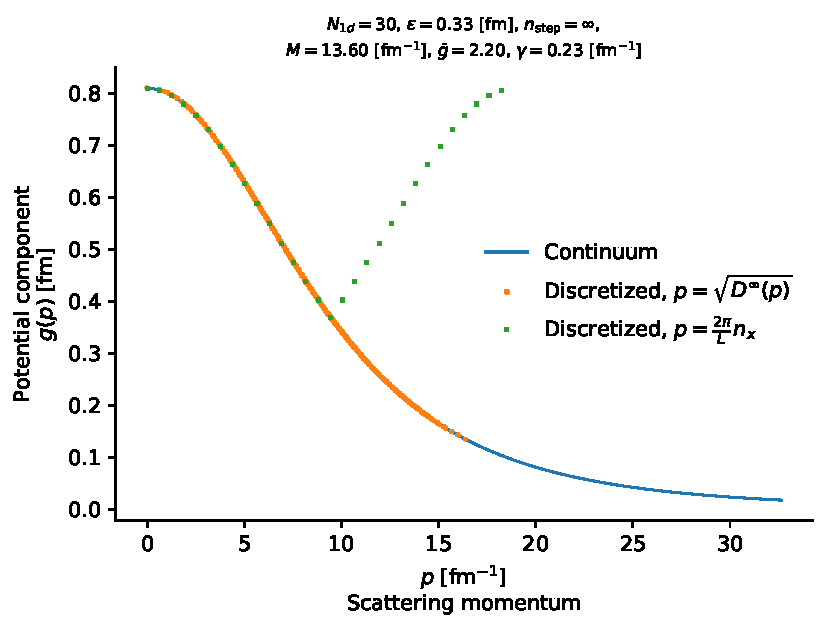
\includegraphics[width=0.7\textwidth]{figs/potential-component.pdf}
\caption{
	\label{fig:potential-component}
	Separable component $g(p)$ of the potential $V(p', p) = -g(p') g(p)$ for chosen lattice parameters agrees at available lattice momenta with continuum infinite volume counterpart.
	Ultra violet momenta part is covered up till $g(p) \sim 0.1$ fm.
}
\end{figure*}

\begin{figure*}[!htb]
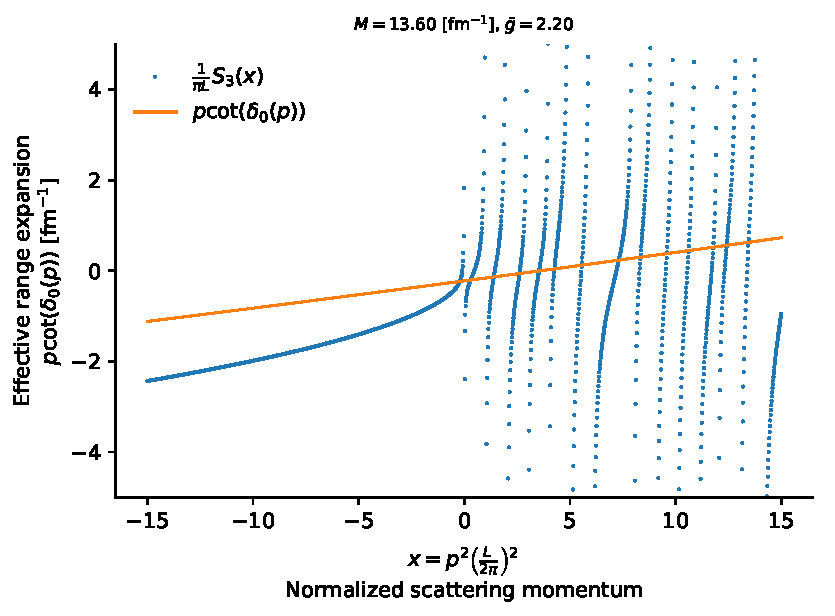
\includegraphics[width=0.7\textwidth]{figs/pcotdelta-intersection.pdf}
\caption{
	\label{fig:pcotdelta-intersection}
	Continuum infinite volume effective range expansion has well defined intersection with zeta function for given parameters.
	E.g., only one intersection at negative energies is given and allows for an extraction of a unique ground state.
}
\end{figure*}


\begin{figure*}[!htb]
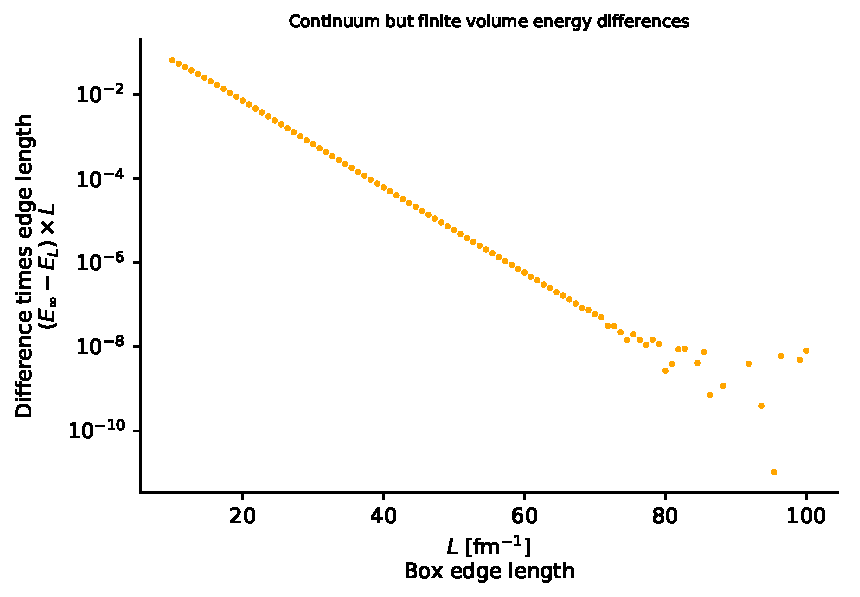
\includegraphics[width=0.7\textwidth]{figs/finite-volume-energy-difference.pdf}
\caption{
	\label{fig:finite-volume-energy-difference}
	Difference of continuum infinite volume energies and continuum finite volume energies times box length, extracted from the first intersection of the zeta function and the effective range expansion (see fig.~\ref{fig:pcotdelta-intersection}), decays exponentially.
	Numerical precision disturbs the result at $10^{-8}$.
}
\end{figure*}

For the chosen potential, solutions can be extracted reliably for the following parameters
\begin{itemize}
	\item Infinite volume continuum ground state energy $E_0 = - 2.225$ MeV.
	\item Finite volume box length $L = 10$ fm.
	\item Potential parameter $M = 20 m_\pi$ (this turns the potential more into a smeared delta function than into a pion exchange).
		This parameter is also fixed in discrete finite volume ("constant of nature") and only $\bar g$ will be adjusted.
\end{itemize}

\subsection{How to pin down finite volume lattice potential parameters?}
How does one implement the potential in a discrete finite volume?
Or more specifically, how to estimate the potential coefficients?
In the following content, I will present three different ideas which take different inputs and try to predict the effective range expansion.
Is there a well behaved way to solve the problem without knowing analytic relations between potential parameters and observables?

\begin{itemize}
	\item Use all known continuum infinite volume parameters to reproduce the result on the lattice.
		Technically this cannot be done for more complex potentials (see fig.~\ref{fig:long-range-ere-v-inf-cont}). 
	\item Solve the discrete finite volume Schrödinger equation to fit $\bar g$ to the continuum infinite volume ground state for each lattice spacing and finite volume.
		Compute phase shifts for each fitted $\bar g$ and observe the convergence pattern against "experimental" results (see fig.~\ref{fig:long-range-ere-v-fit}).
	\item Use "experimental" phase shifts to compute continuum finite volume energies.
		Fit $\bar g$ to the continuum finite volume ground state.
		Compute phase shifts for each fitted $\bar g$ and observe the convergence pattern against "experimental" results (see fig.~\ref{fig:long-range-ere-v-lat}).
\end{itemize}

\begin{figure*}[!htb]
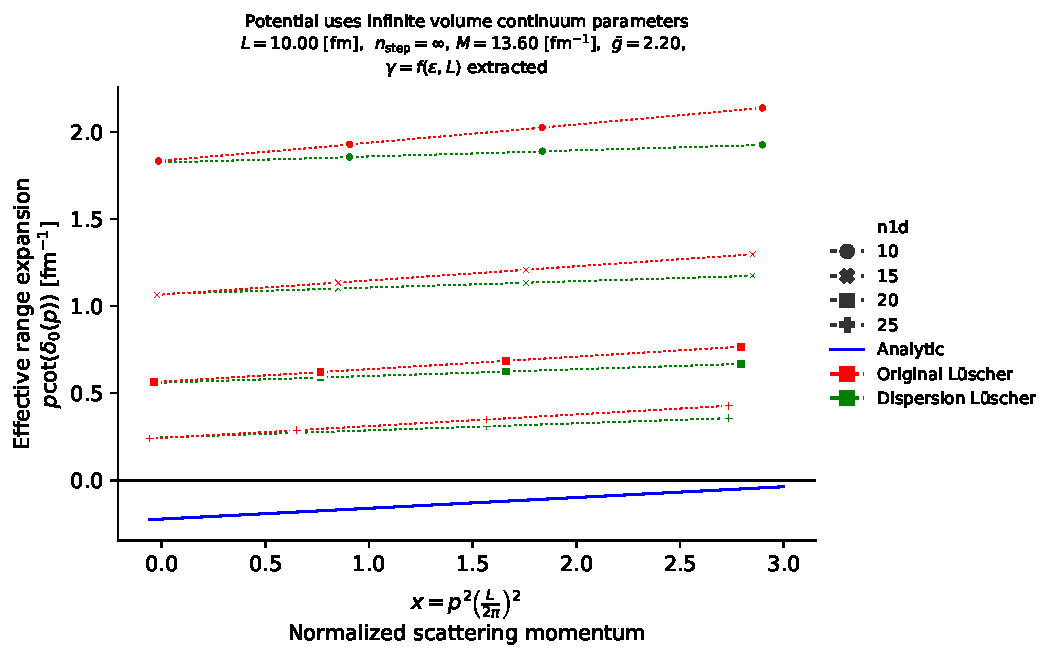
\includegraphics[width=0.7\textwidth]{figs/long-range-ere-v-inf-cont.pdf}
\caption{
	\label{fig:long-range-ere-v-inf-cont}
	Infinite volume continuum parameters were fed into the finite volume lattice potential from which the energy levels were used to compute the effective range expansion.
	The difference between the standard Lüscher phase shift extraction (red markers) and the modified dispersion Lüscher extraction (green markers) is only visible at large normalized scattering momenta $x$.
	For few lattice nodes (large lattice spacings), the extracted ERE does not agree well with the analytic result.
	But for more lattice nodes (finer discretizations), the extracted ERE seemingly converges against the analytic result and the difference between original and dispersion Lüscher shrinks as well.
}
\end{figure*}

\begin{figure*}[!htb]
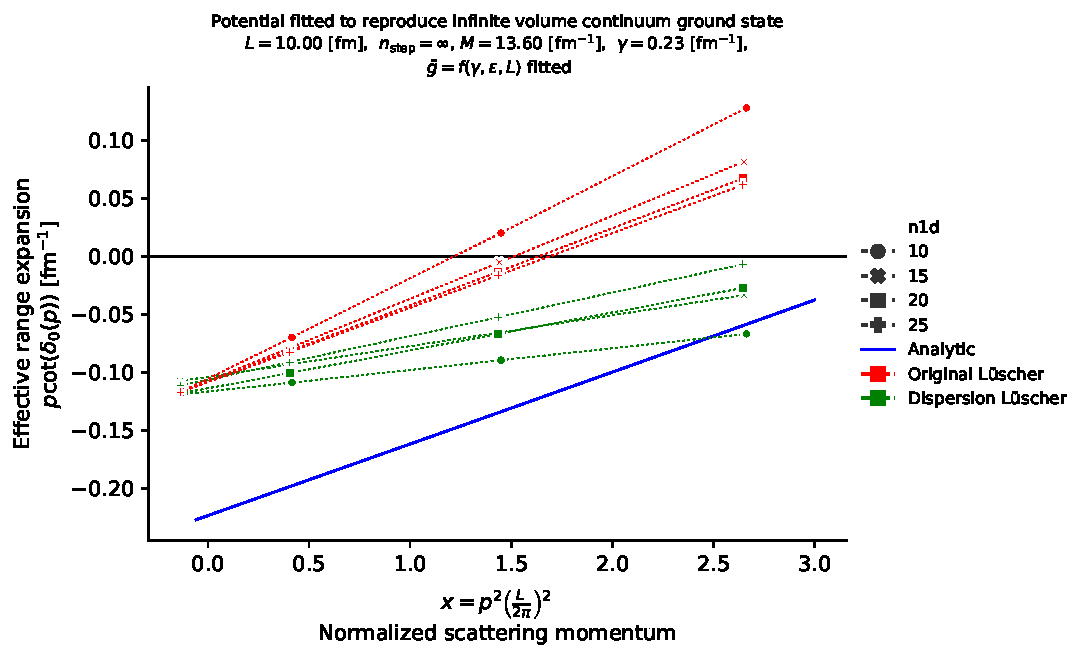
\includegraphics[width=0.7\textwidth]{figs/long-range-ere-v-fit.pdf}
\caption{
	\label{fig:long-range-ere-v-fit}
	Infinite volume continuum energy was used to fit finite volume lattice potential.
	ERE was extracted after fit.
	The difference between the standard Lüscher phase shift extraction (red markers) and the modified dispersion Lüscher extraction (green markers) is small at small $x$ but increases more drastically for large $x$ as in the "known parameter case" (see fig~\ref{fig:long-range-ere-v-inf-cont}).
	For all discretizations, the original Lüscher results agree with themselves at the smallest $x$ because the fit requires each $x$ to be the same and original Lüscher does not provide different different zeta functions for different discretizations.
	This is different for dispersion Lüscher.
	The $y$-values are different because one uses dispersion dependent zeta functions.
	The standard Lüscher has a nice internal convergence pattern (the finer discretization, the smaller the changes of the ERE) but it seemingly converges against a completely wrong value.
	The dispersion Lüscher convergence pattern seems more random (big step, small step, big step in directions of smaller lattice spacing).
	It is not obvious if dispersion Lüscher and standard Lüscher will converge against the same dispersion relation, but it seems quite reasonable to assume that both approaches will not converge against the analytical result.
}
\end{figure*}

\begin{figure*}[!htb]
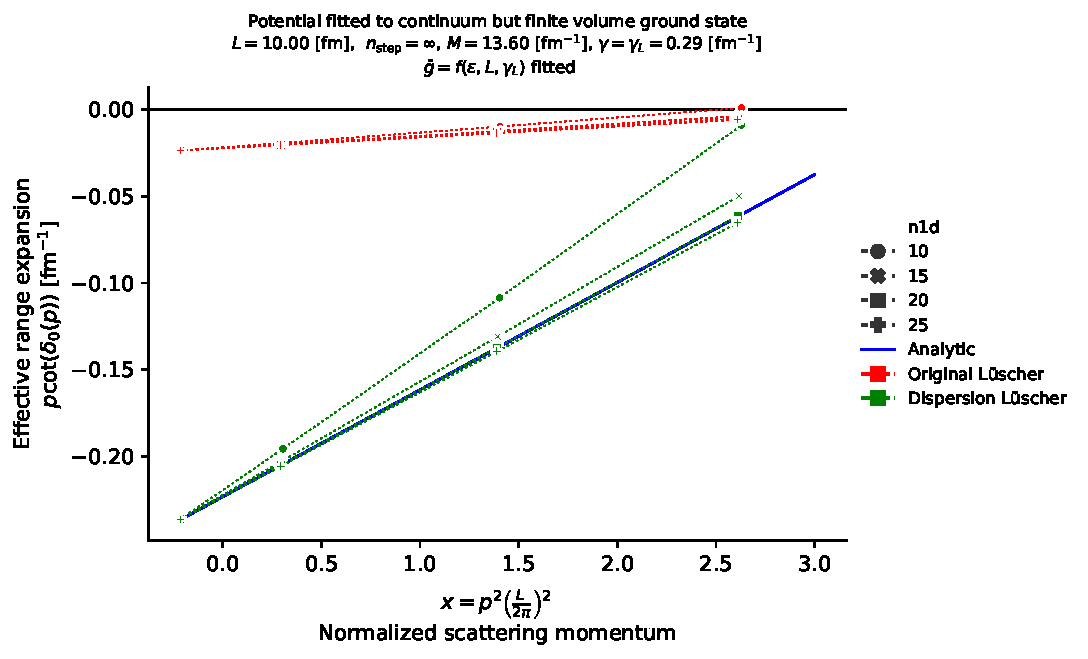
\includegraphics[width=0.7\textwidth]{figs/long-range-ere-v-lat.pdf}
\caption{
	\label{fig:long-range-ere-v-lat}
	First, the finite volume continuum energy was computed using the "experimental" ERE.
	Next the finite volume ground state used to fit the finite volume lattice potential.
	This means that discretization effects were correlated with the potential.
	The ERE was extracted after fit.
	The difference between the standard Lüscher phase shift extraction (red markers) and the modified dispersion Lüscher extraction (green markers) is drastic.
	For all discretizations, again the original Lüscher results agree with themselves at the smallest $x$.
	The standard Lüscher has again a nice internal convergence pattern but still it seemingly converges against a completely wrong value.
	In this case, the dispersion Lüscher results at small $x$ are on top of each other.
	The dispersion Lüscher convergence pattern seems well behaved such that the smaller the lattice spacing, the smaller the changes.
	Also, dispersion Lüscher results now seem to covnverge against the continuum infinite volume counterpart.
}
\end{figure*}

\subsubsection{Questions and conclusions}

\begin{itemize}
	\item Give me a night to sleep over the results.
	\item One big question I have is: assuming that things actually work, why do we still see a convergence pattern in fig.~\ref{fig:long-range-ere-v-lat}?
	\item It seems to me that the best way of fixing coefficients is mapping the ERE to coefficients and computing binding energies.
\end{itemize}


\end{document}